\documentclass[a4j]{jarticle}
\usepackage[dvipdfmx]{graphicx}	%必要
\usepackage[dvipdfmx]{color}	%必要
\usepackage{url}				%実験のテンプレに記載

\setlength{\headsep}{-5mm}
\setlength{\oddsidemargin}{0mm}
\setlength{\textwidth}{165mm}
\setlength{\textheight}{230mm}
\setlength{\footskip}{20mm}


\begin{document}
\section{情報・金銭の流れ}

\subsection{情報の流れ}
子育て支援アプリの利用による情報の流れを図\ref{info}に示します。		%子育て支援(アプリorシステム)?

アプリ内で提供されているゲームで遊ぶと結果が記録されます。記録した結果は、親がいつでも確認することができます。親は子育て支援アプリを利用している他の親と、子育てに関する情報の共有を行います。アプリの機能に不具合があった場合は、利用者が管理人に連絡できるようになっています。管理人は新しいゲームなどの追加コンテンツの提供、アプリの修正を行います。アプリに広告を提供できる企業は、子育てや幼児教育に関する事業を行っている企業に限定します。これによりアプリの利用者は、子育てに関連する有益な情報を広告からも得ることができます。
%今井は「アプリ」と略して記述しました。統一すべき。
\begin{figure}[h]
  \begin{center}
    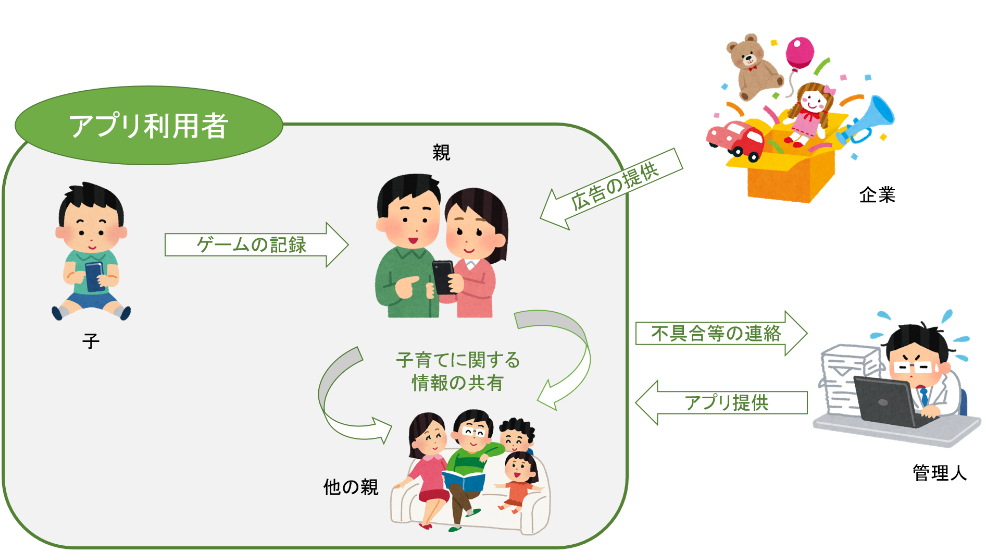
\includegraphics[width = 14cm, height = 9cm]{section5_info.png}
    \caption{情報の流れ}
    \label{info}
  \end{center}
\end{figure}

\newpage
\subsection{金銭の流れ}
子育て支援アプリの利用による金銭の流れを図\ref{money}に示します。

子育て支援アプリは有料提供を行います。アプリ内で広告を提供している企業は、管理人に広告費用を支払います。アプリ利用者がアプリ内に表示されている広告商品の購入等を行うことにより、広告を提供している企業側の売上が見込めます。

\begin{figure}[h]
  \begin{center}
    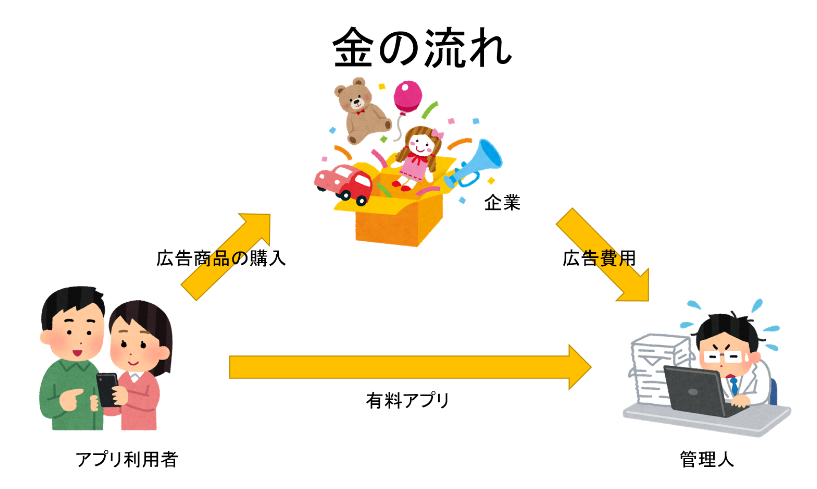
\includegraphics[width = 14cm, height = 9cm]{section5_money.png}
    \caption{金銭の流れ}
    \label{money}
  \end{center}
\end{figure}


\end{document}

